\subsection{Sentence View}
\label{sec:sentence}
% Once an exploration cycle started, the experts need to examine the premise and hypothesis sentence the current example.
As illustrated in Fig.~\ref{fig:sentenceView}, the sentence view shows the premise and hypothesis sentence in (c) and (d).
%
To facilitate the analysis task (\textbf{T1}), we employ an automate sentence perturbation scheme that replaces \emph{nouns} and \emph{verbs} by their synonymous in the wordNet~\cite{Miller1995} (the standard lexical database for NLP applications).
%
When the perturbation is applied to either of the sentences, the replaced words are highlighted in blue (see Fig~\ref{fig:modelPipeline}(e) ) to signal the modification made to the original sentence.

\begin{figure}[htbp]
\centering
\vspace{-2mm}
 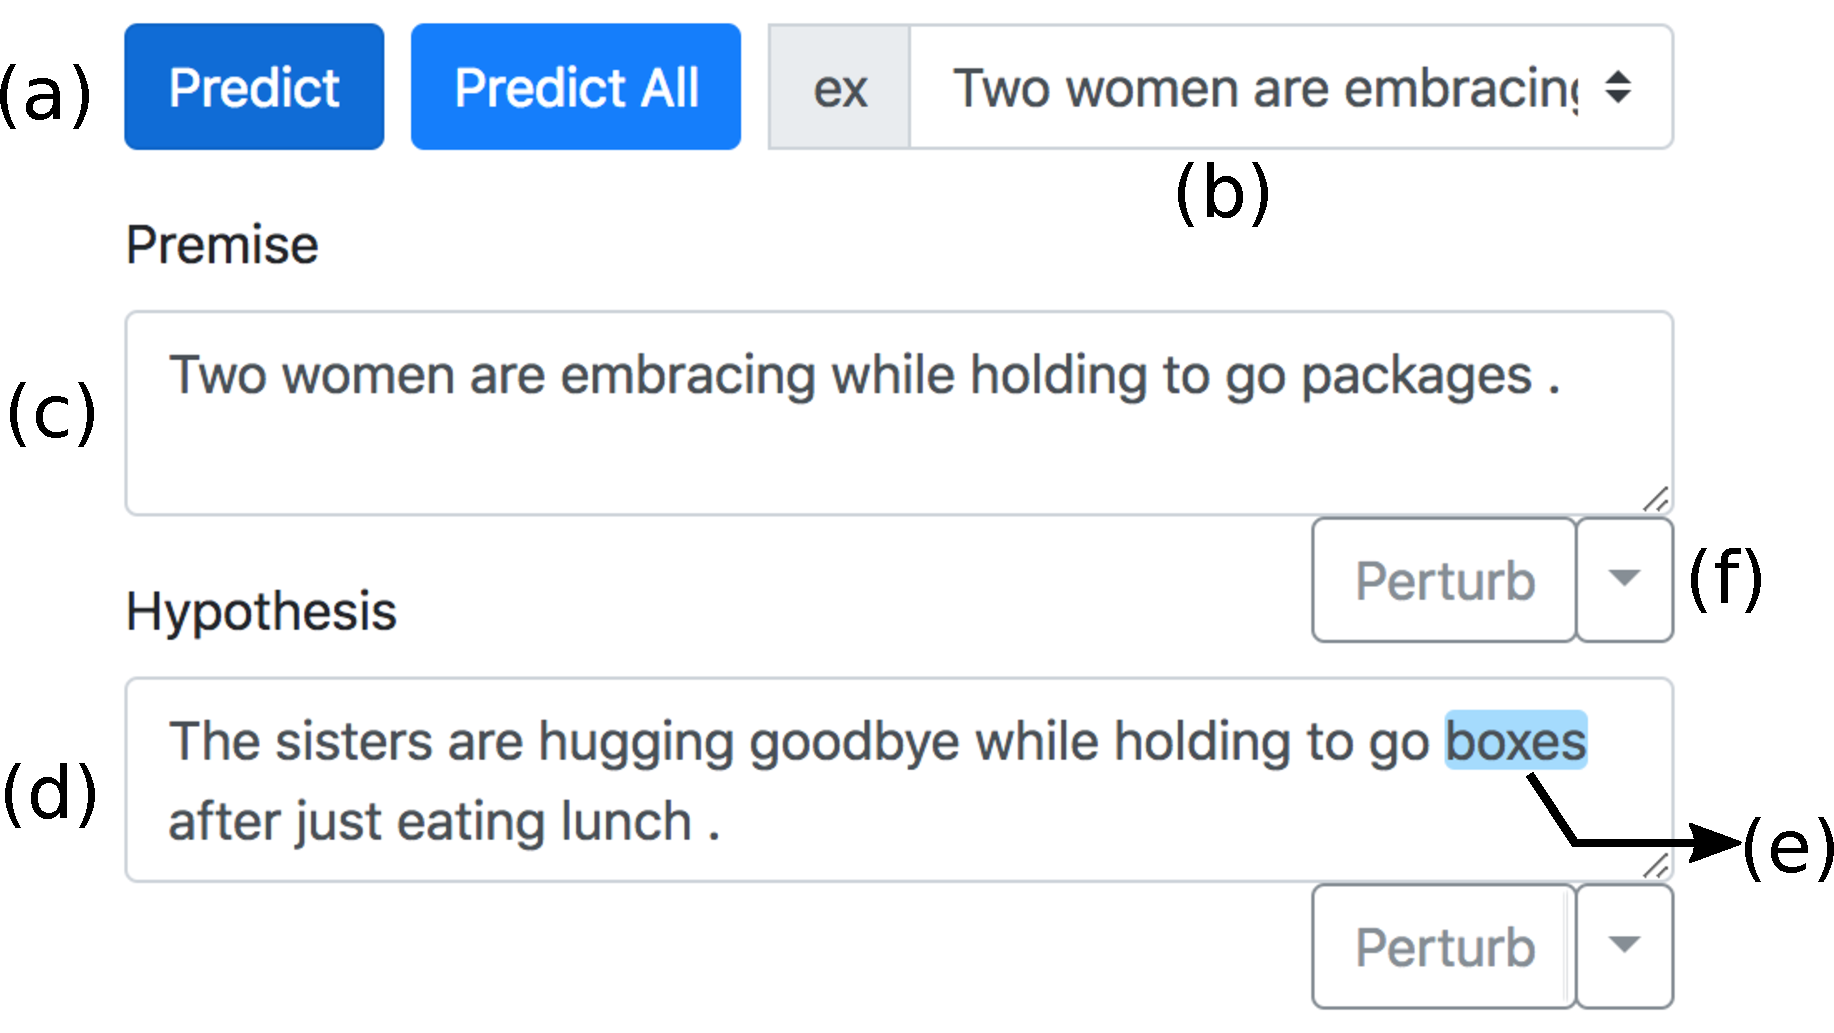
\includegraphics[width=0.95\linewidth]{sentenceView}
 \vspace{-2mm}
 \caption{
 Sentence view shows the premise (c) and the hypothesis (d) sentence pair. The word that replaces the word in the original text is highlighted in blue (e).
 The \emph{Predict} and \emph{Predict All} controls (a) correspond to predicting the currently displayed sentence pairs and predicting all combinations of perturbed premise and hypothesis, respectively.
 Previous explored original sentence are stored in the dropdown list (d) that allow the user to revisit previous examined sentence.
}
\label{fig:sentenceView}
\end{figure}

At the top left of the view, the two controls \emph{Predict} and \emph{Predict All} (a) correspond to predicting the currently displayed sentence pairs and predict all combinations of perturbed premise and hypothesis, respectively.
%
To avoid the situation where both sentences are perturbed, we ensure that only one perturbation per sentence pair (i.e., we use original premise if the hypothesis is perturbed, or use original hypothesis if the premise is perturbed).
%%% sentence perturbation %%%%
The previous explored original sentences are stored in the dropdown list (see Fig.~\ref{fig:sentenceView}(b)) that allow the user to revisit examined examples.
Also, the user can type any sentences or modified existing text in the text areas (Fig.~\ref{fig:sentenceView}(c)(d)) to accommodate user defined input.



%\begin{itemize}
%\item Examine perturbed pair
%\item See which word is perturbed in a sentence
%\item Add to existing example collection
%\end{itemize}
